  \mysection{Whispers}{arcana-whispers}


    Whispers are the disciplines, incantations, hedge magic, illusion, sleight-of-hand, and minor telepathy that constitute the \mybold{Left Hand Path}.  Passed down through instruction, ancient books, and word-of-mouth, Whispers allow you to trick reality into doing what you want.

    Rolling your \KNAVE should only be required by the Arbiter if the difference between success and failure would be interesting, or when the attempt shouldn't be an automatic success.  Your skill in each of the four Whispers is represented by one of the following \STATIC die, called a \KNAVE.  If you are "Untrained" in one of the Whispers, it means you know only the bare details; you would only succeed if the difference between success and failure would be uninteresting or an automatic success.

    \mytable{X r}{
      \thead{Rank} & \thead{\KNAVE} \\
    }{
      Untrained  & 1 \\
      Apprentice & d4 \STATIC \\
      Footpad & d6 \STATIC \\
      Sharper & d8 \STATIC \\
      Master & d10 \STATIC \\
    }

    You may buy additional ranks in a Whisper when you \mylink{advance in level}{advancement-leveling}

    You must be unarmored or wearing \mylink{Light Armor}{gear-armor} to use your Whispers.  You cannot perform Whispers while using a shield.   Using a Whisper in combat is a \mylink{Basic Maneuver}{combat-basic-maneuver}.  Finally, Whispers require verbalization; you must be able to speak in order to use a Whisper (a common punishment for thieves is to cut out their tongues).

    \example {
        \RB: \KNAVE + Modifiers vs. Target
    } 



    If the Arbiter decides the roll is required, she will set a Target (a number between 2 and 9) for the roll (details on difficulty are found in the Arbiter's section on \mylink{Knavery}{arbiter-knave}).  \RB than this number using your \KNAVE (ties go to the Adventurer!)

    You may use your \LUCK to affect your \KNAVE roll, but it can never provide more than a +4 Modifier.



    \explain {
      Flink Lighthand is 3rd level and a Footpad in the Whispers of Sun Wukong (so he has d6 \KNAVE and d6 \LUCK), and he's robbing a crypt.  Creeping down a hallway he peeks through the broken door of an antechamber, and sees the glint of gold at the far end.  Flink's sixth-sense is tingling though, and he asks the Arbiter if he sees any traps in here.  The Arbiter knows there's a cunning poisoned spear trap in the room and assigns a Target of 4/2 to it (4 to find it and 2 to disarm it).  Flink rolls his \KNAVE and gets a 4 - he smells a whiff of tarantula venom in the air, and the large flagstone just inside the door seems to shimmer for a moment.  Bending close to the flagstone that would release the trap, Flink whispers to it and asks it to lock in place.  He rolls again ... and gets a 1!  Thinking quickly, Flink rolls his \LUCK and rolls a 4.  He adds 4 to his roll, making it a 5.  Lucky break - he mixed up the words of the Whisper, but it worked out better than he hoped. \\~ \\~
     Later, Flink finds himself in a spot where he has to climb a rocky cliff to continue his journey.  Flink is "Untrained" in the Whispers of Anne Bonny, but the Arbiter decides that the difference between success and failure isn't interesting at this point of the adventure (she'd rather get him to the surprises she has on the other side!).  Flink's natural ability as a Knave is enough for him to scamper up the rock face.  If the Arbiter felt that this was difficult enough to not be automatic, Flink could still roll his \LUCK and add it to his rank of 1 (Untrained) to try to get up the wall...

    }

  \begin{center}
  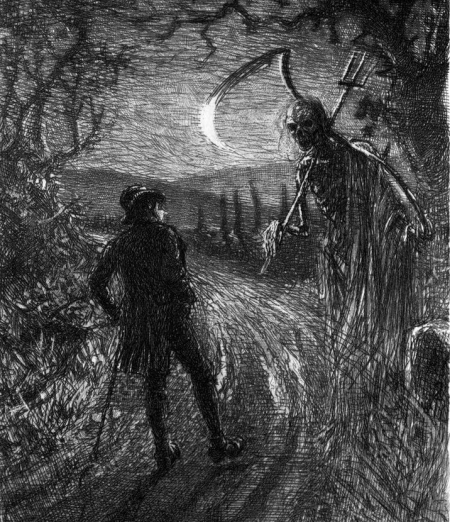
\includegraphics[scale=.5]{Spectre}
  \end{center}




    \mysubsection{Whispers of Anne Bonny}{knave-whisper-ann-bonny}

    Also known as The Swashbuckler, Anne Bonny's instructions show the ways to scale impenetrable fortresses, icy cliffs, and wizard's towers; swing from ropes and vines; disguise yourself to escape patrolling soldiers or to get past armed guards; and forge documents to start wars or gain access to restricted areas. If you are a student of the Whispers of Anne Bonny, a Knave's Sword gains both the Rend and Cleave ability in your capable hands.

    \mysubsection{Whispers of Br'er Rabbit}{knave-whisper-brer-rabbit}

    Br'er Rabbit (The Curious) knows a thing or two about tight squeezes.  His Whispers can help you remove items from pockets without anyone seeing; perform sleight-of-hand, ventriloquism, and distraction to befuddle your marks; escape from ropes and manacles; and cast spells from Fetishes.  If you are a student of the Whispers of Br'er Rabbit, you can turn Invisible (as the spell) once per Session.

    When casting spells from a Fetish, you roll your \KNAVE for the Whispers of Br'er Rabbit instead of Blood Dice.  You can add the result of a \LUCK to this roll as well. The difficulty of reading a spell off a specific Fetish is up to the Arbiter, but the difficulty should default to "automatic"  

    \mysubsection{Whispers of Sun Wukong}{knave-whisper-sun-wukong}

    Sun Wukong is known as The Thief.  His teachings show the secret ways of hiding things on your person so they are difficult to find; uncovering and understanding the mechanisms of traps, snares, and Inscribed Sigils and chide them into disarming themselves; and opening locked chests, doors, and prisons.  If you are a student of the Whispers of Sun Wukong, you can make a sack, bag, or satchel into a Hammerspace Bag.  You can only have 1 Hammerspace Bag in existence at a time.

    \explain {
      The \mybold{Hammerspace Bag} can contain up to 12 Significant Items.  Searching for a Significant Item is a 1-in-(number of items) chance of finding it per Moment i.e. if you have 6 Significant Items in the bag, you have a 1-in-6 chance of pulling it out in a Moment.  You can pull out Insignificant Items stored in the bag immediately.  If you die, all of the contents of the bag are immediately ejected
    }




    \mysubsection{Whispers of The Bride}{knave-whisper-the-bride}

    The Bride is known by many names, none of them spoken aloud:  Lady Death, the Banshee, the Viper, etc.  Education in the Whispers of the Bride teaches you the mental tricks, hypnotism, and observation necessary to sneak past (or behind) people without them noticing you, to silence the clink of coins in your pocket and the sound of your breath and heartbeat. In addition, the Bride teaches you the finer points of committing Murder, provided you get \mylink{the Drop}{combat-surprise} . If you are a student of the Whispers of the Bride, you do not need to make \DEX checks for handling Toxins or Acids.

    \cbreak

    \myhighlight{Murder}{knave-murder}

    If you get \mylink{The Drop}{combat-surprise} on someone, you can attempt a Murder.  Murder can only be performed at Close range with a Shortsword, Dagger, Club, or Hand Axe.  Make a standard Fight \RO; if you hit, pick \mybold{one} of the following attacks:

    \dashedbox {
      \mybullet {
        \item \mybold{Cautious:}  You automatically \mylink{Crit}{combat-crits-and-fumbles} (do maximum damage + \LVL).  Any weapon.
        \item \mybold{Reckless:}  You do 3d6 damage.  Any weapon.
        \item \mybold{Bloody:}  You roll damage normally, but the Monster is also Bleeding. Stabbing only.
        \item \mybold{Waylaying:}  You can either roll damage and the Monster is Woozy, or do no damage and the Monster must Save or be Knocked Out.  Bashing only.
      }
    }

   Murder is a Combat Action, so it can't be combined with other Combat Actions (like Florentine). Damage bypasses any Armor or Soak, if applicable (you slip the blade between the Monster's scales / plate mail / chink in carapace). Once you commit a Murder, you no longer have the Drop unless you're able to get out of sight again. Note that Monsters who are Amorphous or immune to surprise cannot be Murdered. 



  \explain {
    Deego Foxears (3rd Level Knave and student of The Bride) and Stalwart Hamhands (3rd Level Sellsword) come around the corner and surprise a clutch of three Ghouls and a necromancer standing at an altar.  The ghouls are Close and the necromancer is Nearby.  The Arbiter rules the ghouls and necromancer are surprised, so Flink has The Drop.  He tries his Fight \RO and succeeds.  He's armed with a Knave Sword and opts to attack "Cautiously".  He deals 11 damage (8 for the sword + \LVL) and stabs a ghoul through the heart before it can react. Stalwart steps up behind him and guts another ghoul with his polearm.  The single remaining ghoul rolls morale and foolishly decides to stay and fight.

    ~\\

    Deego and Stalwart roll Init - Deego rolls well over 20, Stalwart less so (he's wearing plate mail).  Deego takes the opportunity to duck into the shadows to try to get the Drop on the necromancer. The Arbiter gives the difficulty a 3 (2 for the ghoul's \HD; an extra 1 because the ghoul is Close and aware Deego's there, but he's mostly focused on the huge armored guy with a polearm; and no modifier for the necromancer, who's completely absorbed in his ritual). Deego rolls his d6 and gets a 5, and slips out of view.  The Ghoul attacks Stalwart and hits, but Stalwart is able to absorb the damage with his Grit.  The necromancer seems to be trying to finish his ritual and doesn't make a move.  It's Stalwart and Deego's turn; Deego takes another Tactical Maneuver and moves Nearby (right behind the necromancer), while Stalwart engages the remaining ghoul.  Depending on how Init goes the next Moment, Deego will be able to take a Combat Action, and hopefully stop the wizard from releasing some eldritch horror ...
  }

